\documentclass{article}[12pt]
\usepackage{silence}
\usepackage{graphicx}

\hbadness=9999999

\newcommand{\aetitle}{WortEx} % Title of the report
\newcommand{\studentOne}{Artur Schäfer} % Name 1
\newcommand{\studentTwo}{Donatien Leray} % Name 2

\begin{document}
\noindent
Linguistic gaming with Python \hfill \studentOne\\
WS 23/24 \hfill \studentTwo

{\begin{center}
\begin{sffamily}\Huge\bfseries \aetitle \end{sffamily}
\end{center}}


    \section*{Introduction}

    Leaning new words can be pretty boring, so we have created a game to make
    it more exciting. Wortex is a linguistic word game. It is designed to
    challenge players' linguistic skills by letting them write all the words
    they can form out of a given set of letters. In this report, we will
    discuss the objectives, mechanics, and features of the game. Linguistic
    games offer a fun way to improve vocabulary and spelling skills. Wortex is
    implemented in Python and uses the Pygame library for its graphical user
    interface.

    \section*{Objectives}

    The primary objective of Wortex is to form as many words as possible from a
    given set of seven letters. Players must create words of at least three
    letters, up  to the maximum length of seven. \\\\ The more words a player
    forms, the higher their score. To achieve a top score, players should aim
    to construct not only words, that are as long as possible but also rare.
    The game ends if the timer runs out or if the player finds all possible
    words, that can be formed from the set of given letters.

    \section*{Mechanics}

    \subsection*{Menu}

    Upon launching the game, players are greeted with a menu. Here, they can
    choose their preferred language (English or German) and view a scoreboard
    showcasing the highest scores achieved. Player can also decide what
    difficulty level they want to play. The difficulty level changes the time
    the player has to find words. They can choose between easy, medium, hard and
    extreme.


    \begin{figure}[ht]
        \centering
        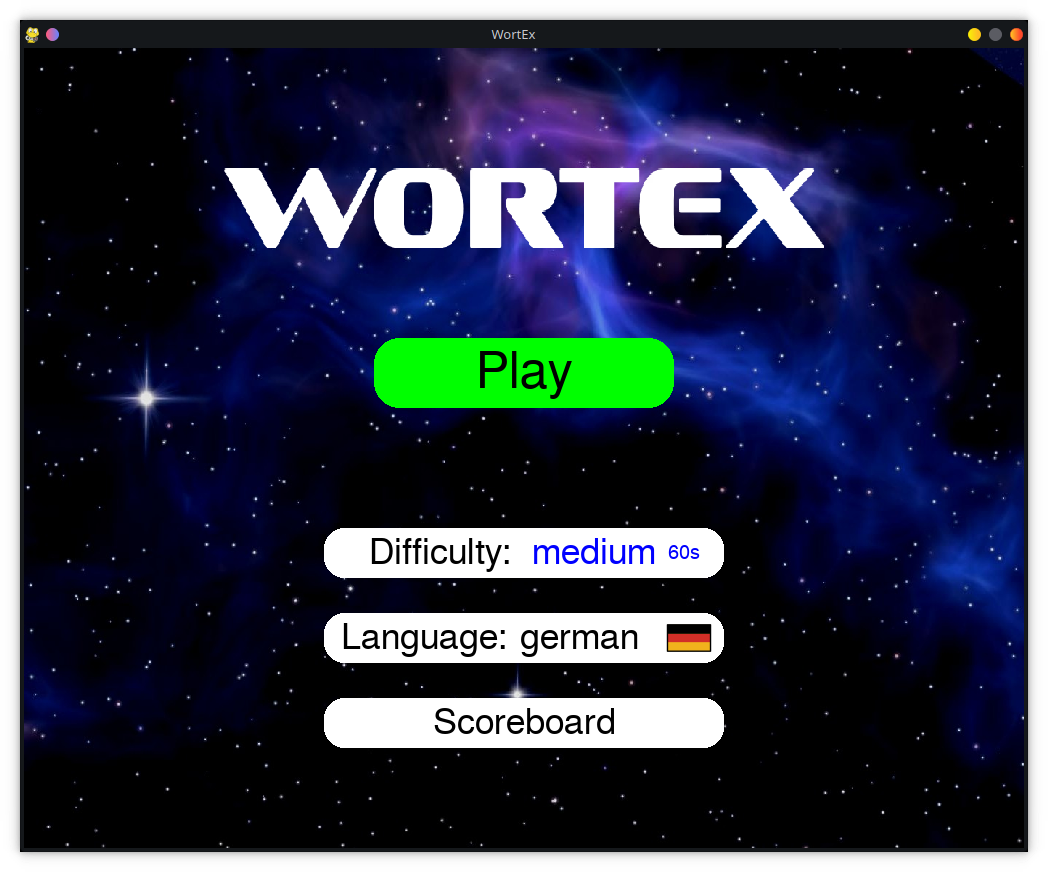
\includegraphics[width=0.5\textwidth]{pictures/menu.png}
        \caption{The main menu of Wortex}
    \end{figure}

    \noindent
    Upon launching Wortex, players are presented with a menu. Here, they can
    choose a language (English or German) they prefer to play with. There is also
    a button to view a scoreboard, which is showcasing the highest scores ever
    achieved. The player also can choose a difficulty level where the time is 
    increased or decreased depending on the level.

    \subsection*{Gameplay}

    After selecting a language and the play button is pressed, the game begins.
    It provides the player with a set of seven letters. On the screen you can
    see a timer, the score, and a list of words that appears if the player
    types a correct word. In the middle there is a circle that represents the
    time and in that circle there are the letters that can be typed to form
    words. Also there is information about how many words can be found in the
    given set. The player can form the words by typing the letters on the
    keyboard. With the escape key, the player can reset his input or by
    deleting the last letter with backspace. After guessing a correct word, the
    input gets cleared and the found word is added to the list of found words.
    If a seven letter word is found, the player gets bonus time to find more
    words. Also if the player guessed a word that is rare, the player gets more
    points than for a common word. There are no penalties for guessing wrong.
    The player is just wasting time that could have been used to find more
    words. 

    
    \begin{figure}[ht]
        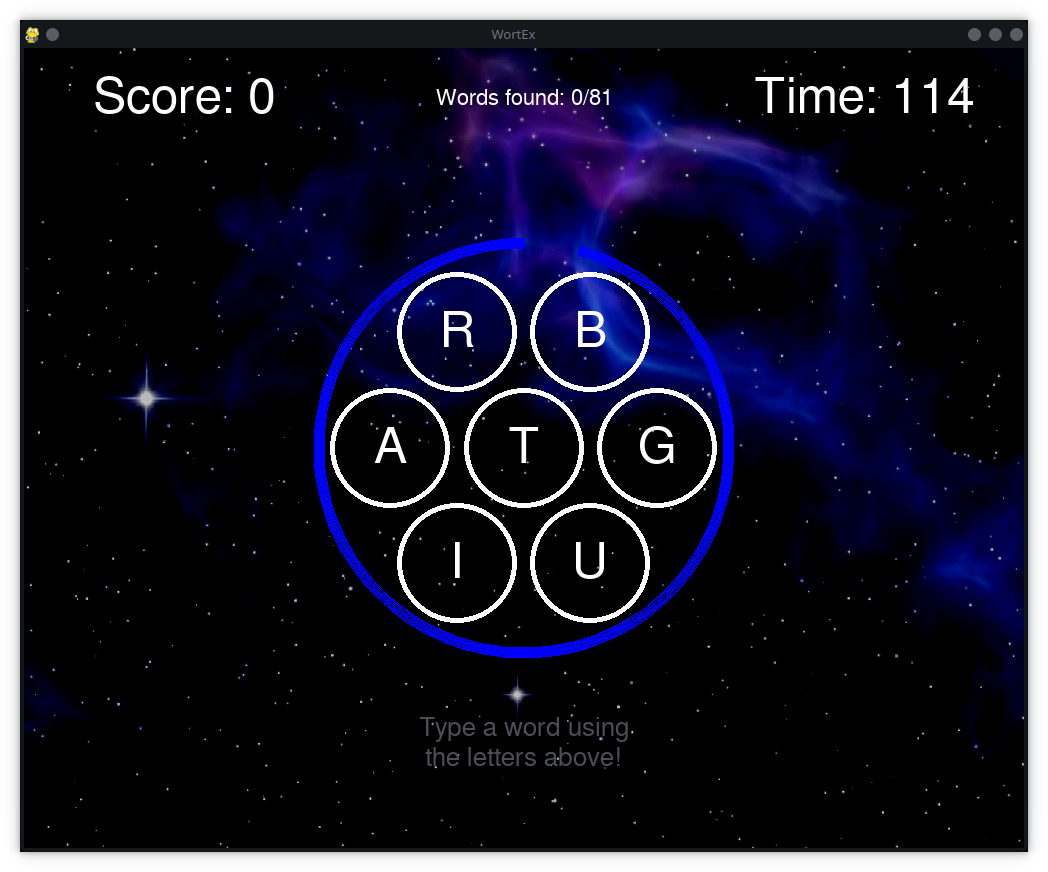
\includegraphics[width=0.49\textwidth]{pictures/gameplay.png}
        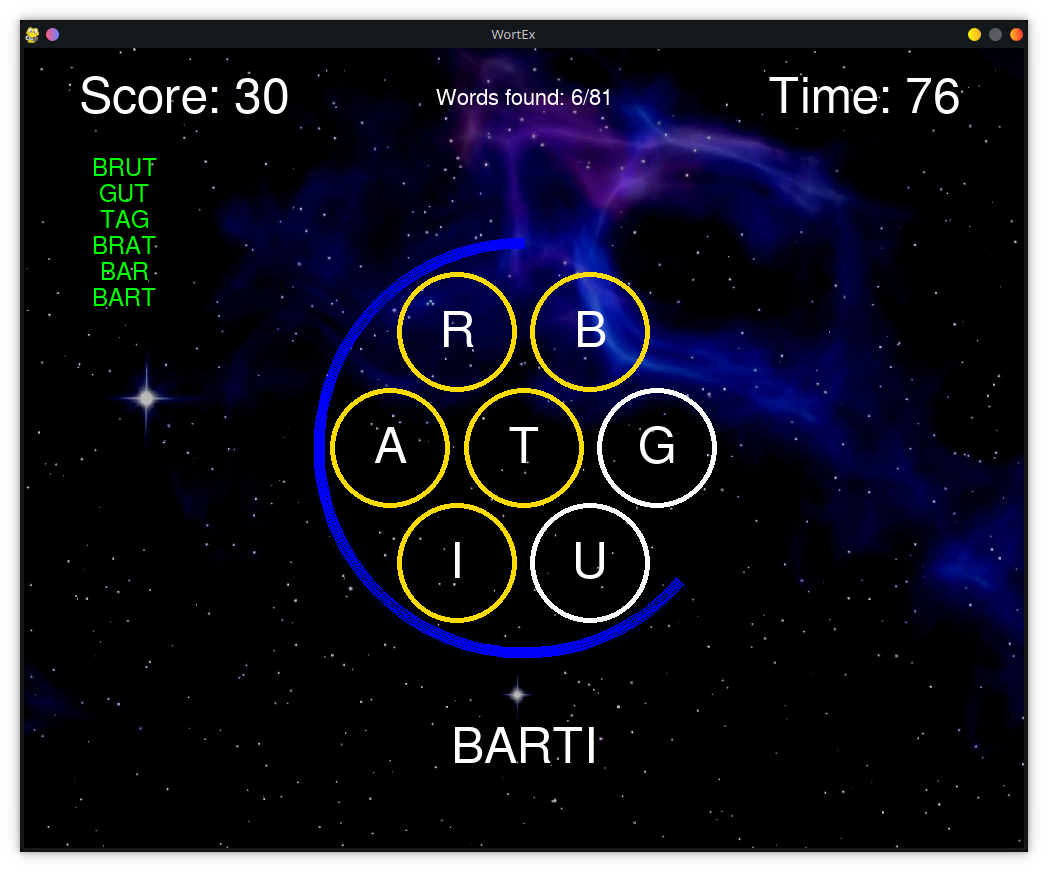
\includegraphics[width=0.49\textwidth]{pictures/mid_game.png}
        \caption{Gameplay of Wortex}
    \end{figure}

    \subsection*{Features}
    
    After the timer runs out or the player achieves to find all possible words,
    the game ends and the player is presented with a screen that shows the
    score and all the words that could be found and also were found by the
    player marked as green. The words can now be clicked on and it opens the
    browser to the definition of the word. In German we open the online Duden
    dictionary and for English the online Oxford dictionary. The player can
    then repeat the process by pressing the play again button or go back to the
    main menu. From the main menu the player can view a leaderboard, which
    shows the highest scores ever achieved. If the game is started again, the
    player gets a new set of seven letters to guess words from.
    We have also impplemented a scorebaord for all the diffrent difficulties.

    \begin{figure}[ht]
        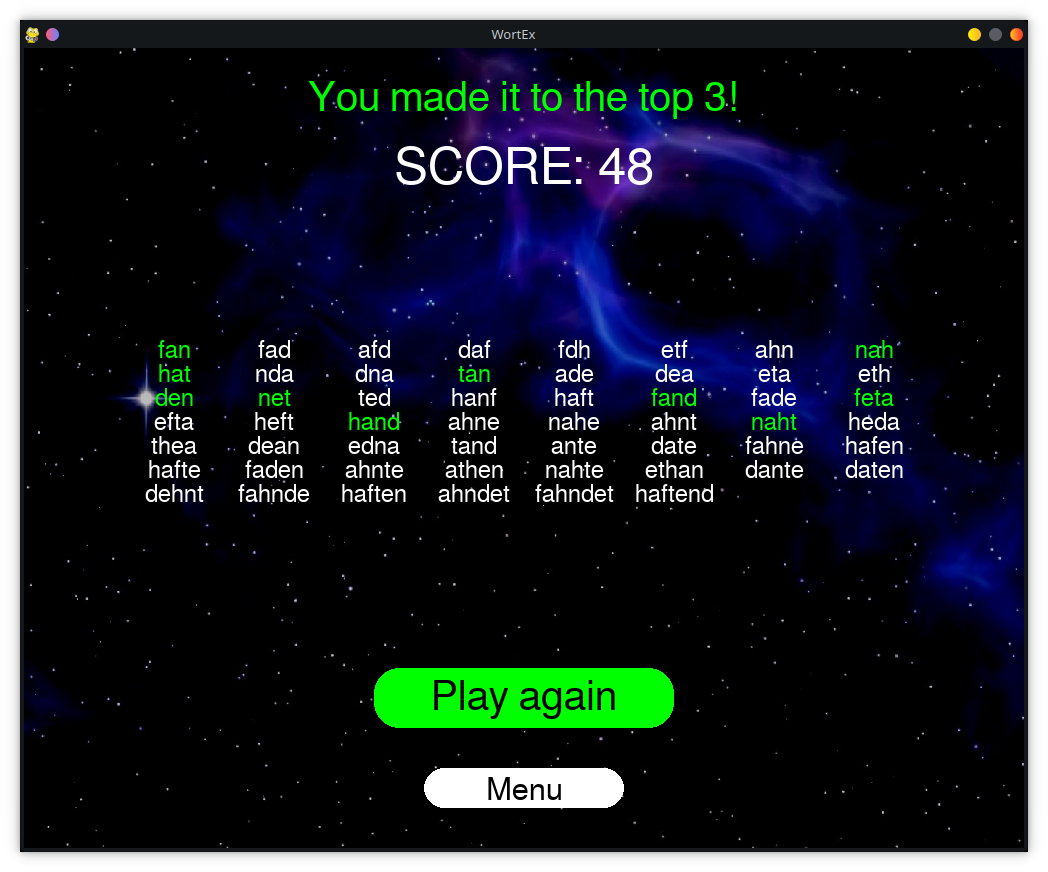
\includegraphics[width=0.49\textwidth]{pictures/endcard.png}
        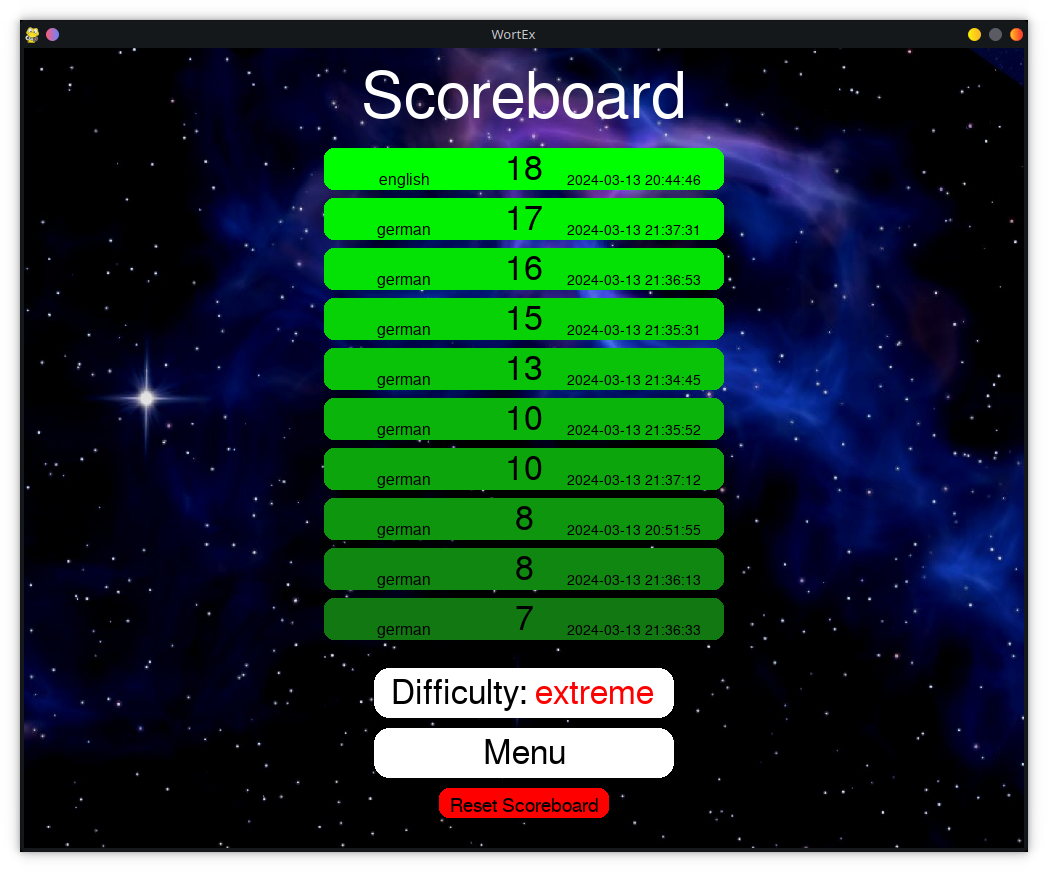
\includegraphics[width=0.49\textwidth]{pictures/scoreboard.png}
        \caption{The end screen of Wortex}
    \end{figure}

    \subsection*{Scoring}

    The score is calculated by the length the frequency of the word of that
    given language. Frequency discribes how often a word appears in a large
    amount of text. The more frequent a word is, the less points the player
    gets for guessing that word. We used a frequency list from a github
    repository that contains about 60000 words and their frequency in the
    German language. We filtered all the words that are out of range of 3 to 7
    letters. Afterwards we calculated the relative frequency of each word and
    used that to calculate the points for each word. Storing this information
    in a database file allows us to just look up the words points and saving us
    to calculate the points on every startup. This is our mathematical model to
    calculate the points for a word:
    \begin{equation}
       P = 1 + \frac{(L - 2) \cdot (1 + 10 \cdot (1 - F))}{15} 
    \end{equation}
    \noindent
    $P$ are the points of a word, $L$ is the length of the word and $F$
    is the relative frequency of the word. The relative frequency is calculated
    by dividing the frequency of the word by the maximum frequency of all words
    in the list. The maximum frequency is the frequency of the most frequent
    word in the list. The points are then multiplied by a factor that is
    calculated by the average points of all words. This factor is used to make
    the points more accurate.  
    \begin{equation}
        f = \frac{\sum_{i=1}^{n} P_i}{n}
    \end{equation}
    We finally round the points and return them as an integer.
    \begin{equation}
        P_i = \left\lfloor P_i \cdot f \right\rfloor
    \end{equation}

    \subsection*{Easter Eggs}

    If the player manages to form the words "Wortex", "Dodo" or "Artur" they
    recieve a bonus of 42 points and gain extra time. Also the look of the game
    changes a bit.

\end{document}
